\section{Results, ablations and errors}
\IfFileExists{tables/classical_results.tex}{\begin{table}[htbp]
\centering\small
\begin{tabular}{@{}lr@{}}
\toprule
Run & Validation log loss \\
\midrule
uniform & 2.6391 \\
markov & 1.7708 \\
current\_row\_logreg & 1.7227 \\
full\_raw & 1.5194 \\
selected\_classical & 1.5193 \\
\bottomrule
\end{tabular}
\caption{Classical results on the shared v2 cutoffs.}
\end{table}
}{
\todo{Insert the classical validation table from the experiment log.}}
\todo{Add deep model validation results and the chosen model's final test result. The brief's reference scores were measured on test and should be labeled separately from local validation.}

\IfFileExists{tables/classical_ablations.tex}{\begin{table}[htbp]
\centering\small
\begin{tabular}{@{}lrrr@{}}
\toprule
Run & Log loss & $\Delta$ vs. raw & 95\% paired CI \\
\midrule
drop\_lags & 1.5274 & +0.0080 & [+0.0048, +0.0112] \\
drop\_counts & 1.5383 & +0.0189 & [+0.0154, +0.0223] \\
drop\_time & 1.5374 & +0.0180 & [+0.0141, +0.0218] \\
drop\_sensors & 1.5219 & +0.0024 & [-0.0005, +0.0055] \\
add\_pair\_back & 1.5413 & +0.0219 & [+0.0169, +0.0269] \\
four\_fit\_cutoffs & 1.5539 & +0.0345 & [+0.0293, +0.0395] \\
temperature & 1.5193 & -0.00011 & [-0.00020, -0.00001] \\
\bottomrule
\end{tabular}
\caption{Ablations against the raw pair-free tree. Intervals resample machines.}
\end{table}
}{
\todo{Report changes in validation loss relative to the full model.}}
\IfFileExists{tables/classical_interpretation.tex}{The local transition table (1.771) and logistic regression (1.723) are close to the brief's test references of 1.81 and 1.75 \cite{brief}. This is a sanity check that the validation cutoffs capture a comparable level of difficulty.

With a cap of 600 rounds, the patience rule triggered in 5 of 5 tuning trials. The inner holdout selected leaves7\_child220\_l2\_10 at its best iteration of 254, after evaluating 274 rounds. Adding back the 196-category event pair changed validation loss by +0.0219. With the pair excluded in both models, dropping the six individual lags changed loss by +0.0080. Dropping sensor history changed loss by +0.0024, with an interval spanning zero. The remaining features include current sensor readings. The sensor history did not show a clear incremental effect. Using four cutoffs per fitting machine changed loss by +0.0345 at the same tree settings.

Temperature scaling fitted \(T=0.9955\) and changed loss by -0.0001, with a paired interval excluding zero. Temperature scaling gave a statistically detectable but negligible gain (about 0.00011 log-loss points). The calibration split selected temperature scaling. For the three rare target classes, the share assigned under 0.5\% probability for the true event was 11.6\% raw and 11.9\% after temperature scaling. Prior blending fitted \(\alpha=0\), so it reproduced the raw probabilities and is omitted from the table. The paired intervals describe these fitted models and do not adjust for multiple comparisons or include variation across refits.
}{}

% Recurrent model results. Included from 04_results.tex.
\subsection{Recurrent model}
We searched one setting at a time around a one-layer GRU with 128 units: 64 or 256 units, two layers, dropout 0.4, learning rate $10^{-3}$ and an LSTM cell. The configuration with the lowest early-stop loss was selected. The validation machines did not influence this choice.
\IfFileExists{tables/gru_tuning.tex}{\begin{table}[htbp]
\centering\small
\begin{tabular}{@{}lrrrrrr@{}}
\toprule
Run & Params & Epoch & Early-stop & $T$ & Val. raw & Val. calibrated \\
\midrule
gru\_h128\_2layers (selected) & 216k & 18 & 1.4629 & 1.010 & 1.4521 & 1.4522 \\
gru\_h128\_drop0.4 & 117k & 38 & 1.4671 & 1.010 & 1.4527 & 1.4528 \\
gru\_h128 & 117k & 24 & 1.4678 & 1.022 & 1.4505 & 1.4506 \\
gru\_h256 & 429k & 13 & 1.4738 & 1.008 & 1.4633 & 1.4633 \\
lstm\_h128 & 150k & 16 & 1.4739 & 1.019 & 1.4540 & 1.4540 \\
gru\_h128\_lr1e-3 & 117k & 24 & 1.4742 & 1.008 & 1.4556 & 1.4557 \\
gru\_h64 & 34k & 40 & 1.4765 & 1.004 & 1.4604 & 1.4604 \\
\bottomrule
\end{tabular}
\caption{Recurrent model search. The selected run has the lowest early-stop loss; validation machines were not used for selection. Validation uses the shared 10,400 cutoffs.}
\end{table}
}{}
\IfFileExists{tables/gru_summary.tex}{The selected model, gru\_h128\_2layers, kept epoch 18 of 22. Temperature scaling fitted $T=1.010$ and moved validation log loss from 1.4521 to 1.4522; accuracy is 53.6\%. Reweighting validation cutoffs to the test length mix gives 1.4464.
}{}
All seven configurations reached validation losses between 1.451 and 1.463, so the recurrent model is not sensitive to these choices. The LSTM (1.454) and GRU (1.451 with one layer, 1.452 with two) performed almost identically, and the two-layer GRU was selected by its early-stop loss. The one-layer GRU scored marginally better on validation, but by less than the spread between training seeds reported below, so the two are equivalent.
\IfFileExists{figures/gru_learning_curve.pdf}{
\begin{figure}[htbp]
\centering
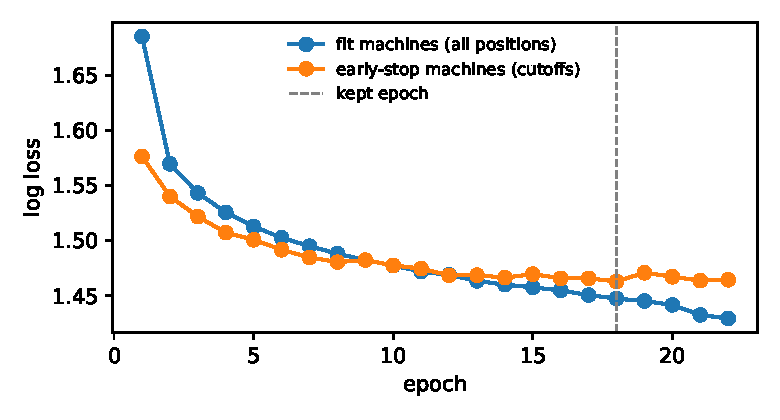
\includegraphics[width=0.62\linewidth]{figures/gru_learning_curve.pdf}
\caption{Training and early-stop log loss of the selected recurrent model.}
\end{figure}}{}

\IfFileExists{tables/gru_ablations.tex}{\begin{table}[htbp]
\centering\small
\begin{tabular}{@{}lrrr@{}}
\toprule
Change from selected GRU & Log loss & $\Delta$ & 95\% paired CI \\
\midrule
Remove time gaps & 1.4603 & +0.0081 & [+0.0024, +0.0137] \\
Remove sensors and missing flags & 1.4565 & +0.0043 & [-0.0011, +0.0097] \\
Remove categorical context & 1.4476 & -0.0046 & [-0.0094, +0.0005] \\
Last 16 events only & 1.5203 & +0.0681 & [+0.0598, +0.0768] \\
Last 64 events only & 1.4573 & +0.0051 & [+0.0003, +0.0098] \\
Add machine-relative sensors & 1.4526 & +0.0004 & [-0.0047, +0.0055] \\
Same model, different seed & 1.4473 & -0.0048 & [-0.0095, -0.0000] \\
No temperature scaling & 1.4521 & -0.0000 & [-0.0003, +0.0002] \\
\bottomrule
\end{tabular}
\caption{One change at a time around the selected recurrent model. Positive $\Delta$ means worse. Intervals resample validation machines.}
\end{table}
}{}
Retraining the selected model with a different seed changed validation loss by $-0.005$. We treat smaller effects as unreliable even when their machine-bootstrap interval excludes zero, because that interval does not include training randomness. History length had by far the largest effect. With only the last 16 events, loss rose by 0.068, while the last 64 events cost only about 0.005. Most of the useful context therefore lies within roughly the last 64 events, but a few events are not enough. Removing time gaps raised loss by 0.008 (95\% CI $[0.002, 0.014]$), the only input group whose removal clearly hurt, consistent with the importance of recency features in the classical model. Removing sensor inputs (+0.004, interval spanning zero) or categorical context ($-0.005$) changed loss by no more than the seed variation. This agrees with the classical result that sensor history adds little beyond the event stream. Machine-relative sensors (+0.0004) gave no gain. Temperature scaling fitted $T=1.01$ and changed loss by less than 0.0003, because the network was already calibrated: predictions made with 80--90\% confidence were correct 85\% of the time.

\IfFileExists{tables/gru_compare.tex}{\begin{table}[htbp]
\centering\small
\begin{tabular}{@{}lrrr@{}}
\toprule
Model (vs. selected GRU) & Log loss & $\Delta$ & 95\% paired CI \\
\midrule
LightGBM & 1.5193 & +0.0672 & [+0.0586, +0.0758] \\
Average of GRU and LightGBM & 1.4593 & +0.0071 & [+0.0027, +0.0115] \\
\bottomrule
\end{tabular}
\caption{Paired comparison on the shared validation cutoffs. The average is exploratory: equal weights, nothing tuned on validation.}
\end{table}
}{}
The selected GRU improves on the tuned LightGBM by 0.067 (95\% CI $[0.059, 0.076]$), larger than any single feature-group effect in the classical ablations. Averaging the two models' probabilities gave 1.459, which is 0.007 worse than the GRU alone. This suggests that LightGBM's hand-made counts and recency features add no information the GRU has not already learned from the raw sequence. A likely reason for the gain is that the GRU sees the exact order and timing of every event and is trained on about 95 prefixes per machine instead of 12 sampled cutoffs.


\subsection{Error analysis}
\IfFileExists{tables/classical_errors.tex}{For the selected classical model, prefixes of 90--129 events had validation log loss 1.532 (\(n=5294\)), versus 1.487 (\(n=1474\)) for 180--250 events. CONTROL\_ALERT had the largest class-average loss (4.626 over 88 examples). The class mix can differ across length buckets. The most common off-diagonal error was MAINTENANCE\_CHECK classified as VIBRATION\_WARNING (305 cases). The largest individual loss was 6.73, on a prefix of 106 events where the model assigned probability 0.00119 to CONTROL\_ALERT.
}{}
\todo{For the selected team model, report validation loss by event class and history length, with sample sizes. Discuss one high-loss error and one frequent confusion. Compare confidence with accuracy for the highest-confidence predictions and explain any evidence of overconfidence.}
